\documentclass[a4paper,12pt]{article}
\usepackage{geometry}
\geometry{a4paper, margin=1in}

\usepackage{amsmath} 
\usepackage{amssymb}
\usepackage{graphicx}
\usepackage{float}
\usepackage[
    colorlinks=true, 
    linkcolor=blue,     
    citecolor=green,    
    urlcolor=blue       
]{hyperref}
\usepackage{booktabs}
\usepackage{caption}
\usepackage[utf8]{inputenc}
\usepackage{subcaption}
\usepackage{tcolorbox}
\usepackage{colortbl}
\usepackage{xcolor}
\usepackage{ragged2e}
\usepackage{algorithm}
\usepackage{algpseudocode}
\usepackage{tikz}
\usetikzlibrary{shapes.geometric, arrows, positioning,shadows}

\bibliographystyle{ieeetr}

\parindent 0px

% Custom Colors
\definecolor{myorange}{rgb}{0.85, 0.49, 0.13}
\definecolor{myblue}{rgb}{0.15, 0.65, 0.90}
\definecolor{mygreen}{rgb}{0.19, 0.82, 0.28}
\definecolor{myred}{rgb}{0.85, 0.11, 0.11}


\begin{document}

\begin{titlepage}
    \begin{center}
        \includegraphics[width=0.5\textwidth]{report images/buet_logo.png} \\ % Replace with your logo file
        \vspace{0.5cm}
        \Large{\textbf{CSE200 - Technical Writing and Presentation}} \\
        \vspace{1cm}
        \Large{\textbf{BANGLADESH UNIVERSITY OF ENGINEERING AND TECHNOLOGY}} \\
        \vspace{0.5cm}
        \large{\textbf{DEPARTMENT OF COMPUTER SCIENCE AND ENGINEERING}} \\
        \vspace{2cm}
        \rule{\linewidth}{0.5mm} \\[0.4cm]
        {\Huge{\textbf{AUTOENCODER}}} \\
        \rule{\linewidth}{0.5mm} \\[2cm]
        {\large{\today}} \\[1cm]
        \vfill
        \begin{tabbing}
            \hspace{5cm} \= \hspace{0.5cm} \kill
            Subsection \> : A2 \\ Group \> : 10 \\
            Nabiha Tahseen \> : 2105031 \\
            Abhishek Roy \> : 2105033 \\
            Fariha Ifrat \> : 2105059 \\
        \end{tabbing}
    \end{center}
\end{titlepage}

\tableofcontents
\listoffigures
\listoftables

\newpage


\begin{center}
    \rule{\linewidth}{0.4mm} \\[1em] % Top line
    \textbf{\Large Autoencoder} \\ % Title
    \rule{\linewidth}{0.4mm} % Bottom line
\end{center}

\vspace{0.5cm}
    
    \begin{center}
        \begin{large}
            \textbf{Abstract} \\[0.5cm]
        \end{large}
        
        \begin{minipage}{0.76\textwidth} % Adjust the width here
            \justify
            Autoencoders are powerful neural networks designed to simplify complex data into smaller, meaningful representations while preserving essential information. They compress data into a compact format (latent space) and reconstruct it, making them ideal for tasks like dimensionality reduction, image denoising, and anomaly detection. Key components include the encoder, latent space, and decoder, each playing a vital role in data processing.
Advanced variations such as Variational Autoencoders (VAEs) and Conditional VAEs (CVAEs) incorporate probabilistic and conditional features, enabling more controlled and meaningful data generation. Denoising autoencoders further extend their utility by effectively cleaning noisy data, with applications in image restoration, speech enhancement, and anomaly detection.
Despite challenges like overfitting and computational demands, continuous advancements are pushing the boundaries of autoencoders. Their growing influence spans diverse fields, from healthcare to creative industries, promising a future of innovative and data-driven solutions.
        \end{minipage}
    \end{center}

\vspace{0.5cm}

%%%%%%%%%%%%%%%%%%%%%%%%%%%%%%%%%%%%%%%%%%%%%%%%%%%%%%%%%%%%%%%%%%%%%%%%%%%%%%%%%%%%%%%%%%%%%%%
                                    % NABIHA TAHSEEN PROMI %
%%%%%%%%%%%%%%%%%%%%%%%%%%%%%%%%%%%%%%%%%%%%%%%%%%%%%%%%%%%%%%%%%%%%%%%%%%%%%%%%%%%%%%%%%%%%%%%

\section{Introduction}  
Autoencoders are a type of neural network specifically designed to handle large and complex data by simplifying it into smaller, more manageable representations. Imagine taking something detailed, like a high-resolution photo or a lengthy dataset, and summarizing it into a compact form while keeping the most essential information intact. This process not only saves storage space but also makes it easier to analyze and work with the data.  

One of the main goals of autoencoders is to reduce the size of the data without losing its important features. After simplifying the data, they can also reconstruct or "rebuild" it back to its original form with minimal differences. This ability makes them extremely useful in a variety of tasks, such as:  
\begin{itemize}
    \item \textbf{Dimensionality Reduction}: Simplifying data with many features into fewer dimensions, making it easier to visualize and analyze.  
    \item \textbf{Image Denoising}: Cleaning up noisy images by learning what the original, noise-free version should look like.  
    \item \textbf{Anomaly Detection}: Identifying unusual or unexpected patterns in data, which is especially helpful in detecting fraud or system errors.  
\end{itemize}  

The primary goal of an autoencoder is to learn how to effectively compress data into a smaller format (known as the \textit{latent representation}) and then accurately reconstruct it. This process focuses on minimizing the \textbf{reconstruction error}, which measures the difference between the original data and the reconstructed data. A well-trained autoencoder ensures that this error is as small as possible, meaning the compressed and reconstructed data are nearly identical to the original.  

In summary, autoencoders are like expert summarizers that make complex data simpler while retaining its core essence, providing a practical solution to many real-world problems in data processing and analysis.  


\section{Data Compression with Autoencoders}  
Autoencoders are highly effective for compressing high-dimensional data into a smaller, more compact representation. For example, consider the following matrix of data:

\begin{equation}
\mathbf{X} = 
\begin{bmatrix}
66 & 98 & 97 & 67 & 79 \\
66 & 27 & 89 & 29 & 24 \\
37 & 92 & 44 & 60 & 54 \\
29 & 53 & 87 & 74 & 17 \\
34 &  2 &  6 & 99 & 63 \\
\end{bmatrix}
\end{equation}

After passing through the encoder, the matrix is compressed into a smaller representation:  

\begin{equation}
\mathbf{Z} = 
\begin{bmatrix}
10 \\
22 \\
34 \\
\end{bmatrix}
\end{equation}

This compression reduces the storage and computation requirements, allowing only the most critical patterns to be retained while discarding redundant details.  

\section{Autoencoder Architecture}
An autoencoder is built using three key components: the \textbf{Encoder}, the \textbf{Latent Space (Bottleneck)}, and the \textbf{Decoder}. Each component plays a critical role in the compression and reconstruction process.  

\begin{figure}[h!]
    \centering
    \includegraphics[width=0.8\textwidth]{report images/architecture.png} % Replace with the correct file name
    \caption{Overview of Autoencoder Architecture showing the Encoder, Latent Space, and Decoder.}
    \label{fig:autoencoder_architecture}
\end{figure}

\subsection{Encoder}  
The \textbf{Encoder} is the first component of an autoencoder. Its primary role is to \textit{compress the input data} into a lower-dimensional representation by identifying the most important features.  
\begin{itemize}
    \item The encoder applies a series of \textbf{nonlinear transformations} to reduce the dimensionality of the input.  
    \item Mathematically, the encoder maps the input \( \mathbf{X} \) to the latent space representation \( \mathbf{Z} \):  
    \[
    \mathbf{Z} = f_{\text{encoder}}(\mathbf{X}; \mathbf{W}_e, \mathbf{b}_e)
    \]
    Here:
    \begin{itemize}
        \item \( \mathbf{X} \): Original input data.  
        \item \( \mathbf{W}_e \): Weights of the encoder.  
        \item \( \mathbf{b}_e \): Bias of the encoder.  
        \item \( f_{\text{encoder}} \): Nonlinear activation function (e.g., ReLU or Sigmoid).  
    \end{itemize}  
    \item This step ensures that the critical features of the input are retained while irrelevant details are discarded.
\end{itemize}

\subsection{Latent Space (Bottleneck)}  
The \textbf{Latent Space}, also known as the \textit{bottleneck}, is the central part of an autoencoder where the \textbf{compressed representation} of the data is stored.  
\begin{itemize}
    \item The size of the latent space is much smaller than the input, which enforces the model to learn the \textit{most essential patterns} in the data.  
    \item Ideally, similar input data points are mapped to nearby regions in the latent space, creating distinct \textbf{clusters} for different classes of data.  
    \item If the dimensionality of the latent space is too low, information loss occurs, leading to poor reconstruction. Conversely, if it is too high, the model may overfit, losing its generalization ability.  
    \item The latent representation \( \mathbf{Z} \) acts as a compressed version of the input:  
    \[
    \mathbf{Z} = [z_1, z_2, \dots, z_n]
    \]
    Where \( n \) is the number of neurons in the bottleneck layer.
\end{itemize}

\subsection{Decoder}  
The \textbf{Decoder} is the final component of an autoencoder. Its goal is to \textit{reconstruct the original data} from the compressed latent representation.  
\begin{itemize}
    \item The decoder performs the reverse operation of the encoder, expanding the low-dimensional latent representation back into the high-dimensional input space.  
    \item Mathematically, the decoder reconstructs the data as:
    \[
    \hat{\mathbf{X}} = f_{\text{decoder}}(\mathbf{Z}; \mathbf{W}_d, \mathbf{b}_d)
    \]
    Here:
    \begin{itemize}
        \item \( \hat{\mathbf{X}} \): Reconstructed data.  
        \item \( \mathbf{W}_d \): Weights of the decoder.  
        \item \( \mathbf{b}_d \): Bias of the decoder.  
        \item \( f_{\text{decoder}} \): Nonlinear activation function.  
    \end{itemize}  
    \item The decoder attempts to minimize the \textbf{reconstruction error}, ensuring the output \( \hat{\mathbf{X}} \) is as close as possible to the input \( \mathbf{X} \).
\end{itemize}



\section{Latent Space Comparison}
The \textit{latent space} is a central component of an autoencoder that determines how well the model compresses and reconstructs data. It acts as the compressed representation of the input, capturing its most essential features. The \textbf{quality of the latent space} depends heavily on its dimensionality, and this affects the organization and separation of data clusters.

\subsection{Lower-Dimensional Latent Space}
When the latent space has a \textbf{low dimensionality}, the following characteristics are observed:
\begin{itemize}
    \item \textbf{Overlapping Clusters}: Data points belonging to different classes often overlap, making it difficult to distinguish between them.
    \item \textbf{Unorganized Representation}: Similar data points may not be placed close together, reducing the efficiency of compression.
    \item \textbf{Information Loss}: Important details of the input data are lost, leading to poor reconstruction.
\end{itemize}

Mathematically, in a lower-dimensional latent space:
\[
\mathbf{Z}_{\text{low}} = [z_1, z_2], \quad \text{where} \; \dim(\mathbf{Z}_{\text{low}}) \ll \dim(\mathbf{X})
\]
The compression ratio is high, but the reconstruction error tends to increase:
\[
L_{\text{low}} = \frac{1}{N} \sum_{i=1}^{N} \|x_i - \hat{x}_i\|^2 \quad \text{(higher error)}
\]

\subsection{Higher-Dimensional Latent Space}
In contrast, a \textbf{higher-dimensional latent space} exhibits the following properties:
\begin{itemize}
    \item \textbf{Distinct Clusters}: Data points belonging to the same class form well-separated, compact clusters, improving the interpretability of the representation.
    \item \textbf{Better Organization}: Similar data points are located close to each other in the latent space.
    \item \textbf{Reduced Information Loss}: More dimensions allow the autoencoder to capture finer details of the input data, resulting in better reconstruction.
\end{itemize}

Mathematically, in a higher-dimensional latent space:
\[
\mathbf{Z}_{\text{high}} = [z_1, z_2, \dots, z_k], \quad \text{where} \; \dim(\mathbf{Z}_{\text{high}}) \approx \dim(\mathbf{X})
\]
Here, the reconstruction error is minimized:
\[
L_{\text{high}} = \frac{1}{N} \sum_{i=1}^{N} \|x_i - \hat{x}_i\|^2 \quad \text{(lower error)}
\]

\subsection{Comparison}
The difference between lower and higher-dimensional latent spaces can be seen in the organization of clusters. In lower dimensions, clusters are overlapping and chaotic, while in higher dimensions, clusters are distinct and well-separated.

\begin{figure}[h!]
    \centering
    \includegraphics[width=1\textwidth]{report images/latentspace.png} % Replace with your file name
    \caption{Comparison of Latent Space: Lower vs Higher Dimensions.}
    \label{fig:latent_space}
\end{figure}


\begin{table}[h]
    \centering
    \begin{tabular}{|c|c|c|}
        \hline
        \textbf{Aspect}                & \textbf{Lower Dimensions}       & \textbf{Higher Dimensions}   \\    
        \hline
        \textbf{Cluster Separation}   & Overlapping clusters            & Distinct clusters                \\
        \hline
        \textbf{Organization}         & Unorganized                     & Well-organized                   \\
        \hline
        \textbf{Reconstruction Error} & High                            & Low                              \\
        \hline
        \textbf{Information Loss}     & Significant                     & Minimal                          \\
        \hline
        \textbf{Interpretability}     & Poor                            & Good                             \\
        \hline
    \end{tabular}
    \caption{Comparison of Lower and Higher-Dimensional Latent Spaces}
    \label{tab:latent_space_comparison}
\end{table}

\section{Loss Function}
The performance of an autoencoder is evaluated using a \textbf{loss function}, which measures the difference between the original input and its reconstructed output. The primary goal during training is to minimize this difference, ensuring that the reconstructed data is as close as possible to the original data.  

One commonly used loss function for autoencoders is the \textit{Mean Squared Error (MSE)}. The MSE quantifies the average squared difference between each input data point \( x_i \) and its reconstructed counterpart \( \hat{x}_i \). Mathematically, it is defined as:
\begin{equation}
L = \frac{1}{N} \sum_{i=1}^{N} \|x_i - \hat{x}_i\|^2
\end{equation}
Where:
\begin{itemize}
    \item \( x_i \): Original input data point.  
    \item \( \hat{x}_i \): Reconstructed data point.  
    \item \( \| \cdot \|^2 \): Squared Euclidean distance, which is computed as:
    \[
    \|x_i - \hat{x}_i\|^2 = \sum_{j=1}^{d} (x_{i,j} - \hat{x}_{i,j})^2
    \]
    Here, \( d \) is the dimensionality of each data point.  
    \item \( N \): Total number of data points in the dataset.  
\end{itemize}

\subsection{Significance of the Loss Function}
The loss function serves as a feedback mechanism during the training process. Here’s how it contributes:
\begin{itemize}
    \item \textbf{Error Quantification}: The loss function calculates the reconstruction error, giving a clear numerical value for how well the autoencoder is performing.  
    \item \textbf{Optimization}: The training algorithm, such as stochastic gradient descent (SGD), uses the computed loss to adjust the encoder and decoder weights iteratively, minimizing the reconstruction error.  
\end{itemize}

\subsection{Interpretation of Loss Values}
\begin{itemize}
    \item A \textbf{high loss value} indicates that the reconstructed output is significantly different from the original input, implying poor compression or reconstruction.  
    \item A \textbf{low loss value} means the reconstructed output closely resembles the original input, showing the autoencoder has effectively learned the data’s underlying patterns.
\end{itemize}

\subsection{Graphical Representation}
The following figure shows how the loss decreases over successive training epochs, reflecting the autoencoder’s improved ability to reconstruct data:

\begin{figure}[h!]
    \centering
    \includegraphics[width=0.8\textwidth]{report images/training.png} % Replace with your file name
    \caption{Loss Curve: Decreasing Reconstruction Error Over Training Epochs.}
    \label{fig:loss_curve}
\end{figure}

\subsection{Practical Implications}
By minimizing the MSE loss, the autoencoder learns to:
\begin{itemize}
    \item \textbf{Preserve Critical Information}: Identify and retain essential features of the input data in the latent space.  
    \item \textbf{Generalize Well}: Avoid overfitting, ensuring the model performs well on unseen data.  
    \item \textbf{Reconstruct Accurately}: Produce outputs that are nearly identical to the inputs, demonstrating effective compression and reconstruction.  
\end{itemize}

\section{Training Process}
The training of an autoencoder is a systematic process aimed at minimizing the \textbf{reconstruction error}. This involves multiple iterations where the model learns to compress and reconstruct data effectively. The entire training process can be broken into the following steps:

\subsection{Steps in the Training Process}
\begin{enumerate}
    \item \textbf{Data Input:} The input data \( \mathbf{X} \) is fed into the model. Each data point in \( \mathbf{X} \) is a high-dimensional representation of the input.
    \item \textbf{Encoding:} The \textbf{encoder} compresses the input data into a \textit{latent representation}, \( \mathbf{Z} \), using the transformation:
    \[
    \mathbf{Z} = f_{\text{encoder}}(\mathbf{X}; \mathbf{W}_e, \mathbf{b}_e)
    \]
    Here:
    \begin{itemize}
        \item \( f_{\text{encoder}} \): Nonlinear transformation function (e.g., ReLU or Sigmoid).
        \item \( \mathbf{W}_e, \mathbf{b}_e \): Weights and biases of the encoder.
    \end{itemize}
    \item \textbf{Decoding}: The \textbf{decoder} reconstructs the original data from the latent representation \( \mathbf{Z} \) using:
    \[
    \hat{\mathbf{X}} = f_{\text{decoder}}(\mathbf{Z}; \mathbf{W}_d, \mathbf{b}_d)
    \]
    Here:
    \begin{itemize}
        \item \( f_{\text{decoder}} \): Nonlinear transformation function.
        \item \( \mathbf{W}_d, \mathbf{b}_d \): Weights and biases of the decoder.
    \end{itemize}
    \item \textbf{Loss Calculation}: The reconstruction error, often computed using \textit{Mean Squared Error (MSE)}, is given by:
    \[
    L = \frac{1}{N} \sum_{i=1}^{N} \|x_i - \hat{x}_i\|^2
    \]
    \item \textbf{Model Update:} The model updates the weights \( \mathbf{W}_e, \mathbf{W}_d \) and biases \( \mathbf{b}_e, \mathbf{b}_d \) using backpropagation and an optimization algorithm such as \textbf{Stochastic Gradient Descent (SGD)}. The objective is to minimize the loss \( L \) over multiple iterations.
\end{enumerate}

\subsection{Optimization Algorithm}
The optimization process adjusts the weights and biases to reduce the reconstruction error. The weight update rule for a parameter \( \theta \) (such as \( \mathbf{W}_e \) or \( \mathbf{W}_d \)) in an epoch is:
\[
\theta \leftarrow \theta - \eta \frac{\partial L}{\partial \theta}
\]
Here:
\begin{itemize}
    \item \( \eta \): Learning rate, which controls the step size of the updates.
    \item \( \frac{\partial L}{\partial \theta} \): Gradient of the loss function with respect to \( \theta \).
\end{itemize}

\subsection{Visualization of Training Process}
The following figure provides a flowchart of the autoencoder training process, showing the encoding, decoding, loss calculation, and weight update steps:

\begin{figure}[h!]
    \centering
    \includegraphics[width=0.9\textwidth]{report images/trainingflowchart.png} % Replace with your file name
    \caption{Training Process of Autoencoder.}
    \label{fig:training_process}
\end{figure}

\subsection{Convergence During Training}
During training, the loss \( L \) decreases as the model learns to better reconstruct the input data. A typical training process is characterized by:
\begin{itemize}
    \item \textbf{Initial Stage}: High loss due to random initialization of weights.
    \item \textbf{Intermediate Stage}: Gradual reduction in loss as the model starts identifying patterns in the data.
    \item \textbf{Final Stage}: Loss plateaus, indicating convergence.
\end{itemize}

\subsection{Table of Training Steps}
The table below summarizes the key steps involved in the training process:

\begin{table}[H]
    \centering
    \caption{Summary of Training Steps in Autoencoder}
    \label{tab:training_steps}
    \begin{tabular}{|c|c|c|}
        \hline
        \textbf{Step} & \textbf{Description} & \textbf{Mathematical Representation} \\ \hline
        Input Data    & Feed input \( \mathbf{X} \) into the model & \( \mathbf{X} \) \\ \hline
        Encoding      & Compress data to latent representation & \( \mathbf{Z} = f_{\text{encoder}}(\mathbf{X}) \) \\ \hline
        Decoding      & Reconstruct input data from \( \mathbf{Z} \) & \( \hat{\mathbf{X}} = f_{\text{decoder}}(\mathbf{Z}) \) \\ \hline
        Loss Calculation & Compute reconstruction error & \( L = \frac{1}{N} \sum \|x_i - \hat{x}_i\|^2 \) \\ \hline
        Weight Update & Adjust model parameters & \( \theta \leftarrow \theta - \eta \frac{\partial L}{\partial \theta} \) \\ \hline
    \end{tabular}
\end{table}


%%%%%%%%%%%%%%%%%%%%%%%%%%%%%%%%%%%%%%%%%%%%%%%%%%%%%%%%%%%%%%%%%%%%%%%%%%%%%%%%%%%%%%%%%%%%%%%
                                    % ABHISHEK ROY %
%%%%%%%%%%%%%%%%%%%%%%%%%%%%%%%%%%%%%%%%%%%%%%%%%%%%%%%%%%%%%%%%%%%%%%%%%%%%%%%%%%%%%%%%%%%%%%%

\section{Importance of Generative Models}

Generative models are essential in machine learning for creating new, realistic data based on learned patterns. Unlike discriminative models, which focus on predictions, generative models replicate the underlying data distribution, enabling tasks like image synthesis, text generation, and data augmentation.

\subsection{Key Applications}
\begin{itemize}
    \item \textbf{Image Synthesis:} Generating realistic faces, styles, or enhancing image quality.
    \item \textbf{Natural Language Processing (NLP):} Producing coherent text or simulating conversations.
    \item \textbf{Medical Imaging:} Creating synthetic scans and augmenting datasets.
    \item \textbf{Data Augmentation:} Addressing data scarcity by generating diverse samples.
\end{itemize}

These models enable control over specific attributes, such as adjusting a smile's intensity in an image. Advanced frameworks like \textbf{Variational Autoencoders (VAEs)} bring structure and flexibility to generative processes, making them invaluable across industries.

\section{Traditional Autoencoders}

\subsection{How Autoencoders Work}
Autoencoders are neural networks designed to learn efficient, lower-dimensional representations of data. They consist of two main components:
\begin{itemize}
    \item \textbf{Encoder:} Compresses input data into a latent representation.
    \item \textbf{Decoder:} Reconstructs the original data from the latent representation.
\end{itemize}

A diagram illustrating the basic structure of an autoencoder is shown in Figure.

\begin{figure}[H]
    \centering
    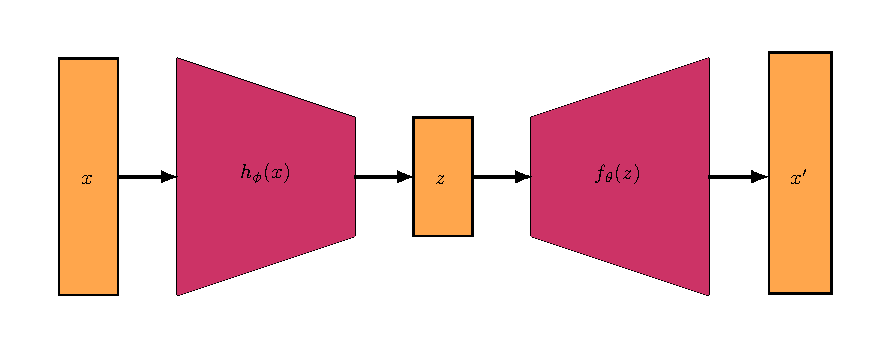
\includegraphics[width=\textwidth]{TIKZ_TEX_FILE/PDFS/basic_auto.pdf}
    \caption{Basic structure of an autoencoder.}
    \label{fig:autoencoder_diagram}
\end{figure}

\subsection{Strengths of Autoencoders}
Autoencoders are effective for dimensionality reduction, noise removal, and feature extraction. They can reconstruct data with high fidelity when trained on representative datasets.

\subsection{Limitations for Generative Tasks}
Despite their strengths, traditional autoencoders face several challenges when used for generative tasks:
\begin{itemize}
    \item \textbf{Overfitting Risk:} Autoencoders tend to memorize the training data and may fail to generalize to unseen data, limiting their usefulness in generating new, diverse samples.
    \item \textbf{Lack of Probabilistic Structure:} Autoencoders do not model uncertainty in the data, making it difficult to generate realistic variations or handle ambiguous inputs.
    \item \textbf{Unstructured Latent Space:} The latent space in autoencoders is often poorly structured and lacks interpretability. This makes it challenging to navigate or control specific attributes in the generated data.
\end{itemize}

\subsection{Implications for Generative Modeling}
These limitations restrict the ability of traditional autoencoders to perform effectively as generative models. The absence of a probabilistic framework and a well-defined latent space often leads to outputs that deviate significantly from the training data distribution, making them unsuitable for advanced generative tasks.

\section{Variational Autoencoders (VAEs)}

\subsection{Origin and Background}
Variational Autoencoders (VAEs) were introduced in the groundbreaking paper \textbf{“Auto-Encoding Variational Bayes”} by \textbf{Kingma} and \textbf{Welling} in 2013. Unlike traditional autoencoders, VAEs are designed to overcome the limitations in generative modeling by incorporating a probabilistic framework. This allows them to generate new data by sampling from a structured latent space, providing both flexibility and control over the generative process.

\begin{figure}[H]
    \centering
    \begin{subfigure}[t]{0.4\textwidth}
        \centering
        \includegraphics[width=\textwidth]{img/kingma.jpg}
        \caption{Diederik P. Kingma, co-author of "Auto-Encoding Variational Bayes".}
        \label{fig:kingma_image}
    \end{subfigure}
    \hspace{3em}
    \begin{subfigure}[t]{0.4\textwidth}
        \centering
        \includegraphics[width=\textwidth]{img/VaePaper.png}
        \caption{First page of the paper "Auto-Encoding Variational Bayes".}
        \label{fig:vae_paper_first_page}
    \end{subfigure}
    \caption{Historical references: Diederik P. Kingma and the foundational VAE paper.}
    \label{fig:vae_references}
\end{figure}


\subsection{How VAEs Work}
VAEs operate by encoding data into a probabilistic latent representation and reconstructing it using a decoder. This section provides an in-depth explanation of each component:

\subsubsection{Input Encoding and Latent Space Representation}
The VAE starts with input data \( x \), such as images, which is mapped into a latent space representation. This process involves the following components:

\paragraph{Encoder:} The encoder transforms the input into two key parameters of a probability distribution:
\begin{itemize}
    \item \textbf{Mean (\( \mu \)) and Log-Variance (\( \log \sigma^2 \))}: These parameters define a Gaussian distribution for each input data point.
    \item The encoder’s role is formalized as:
    \[
    q_\phi(z|x) = \mathcal{N}(z; \mu_\phi(x), \sigma^2_\phi(x))
    \]
    where \( \phi \) represents the parameters of the encoder network.
\end{itemize}

The mean and log-variance enable the generation of latent variables \( z \) through sampling, which is essential for the probabilistic structure of VAEs.

\paragraph{Latent Space Representation:} The latent space is a structured and continuous representation, unlike the unstructured latent space of traditional autoencoders. This space allows for meaningful interpolation and controlled generation of data.

\begin{figure}[H]
    \centering
    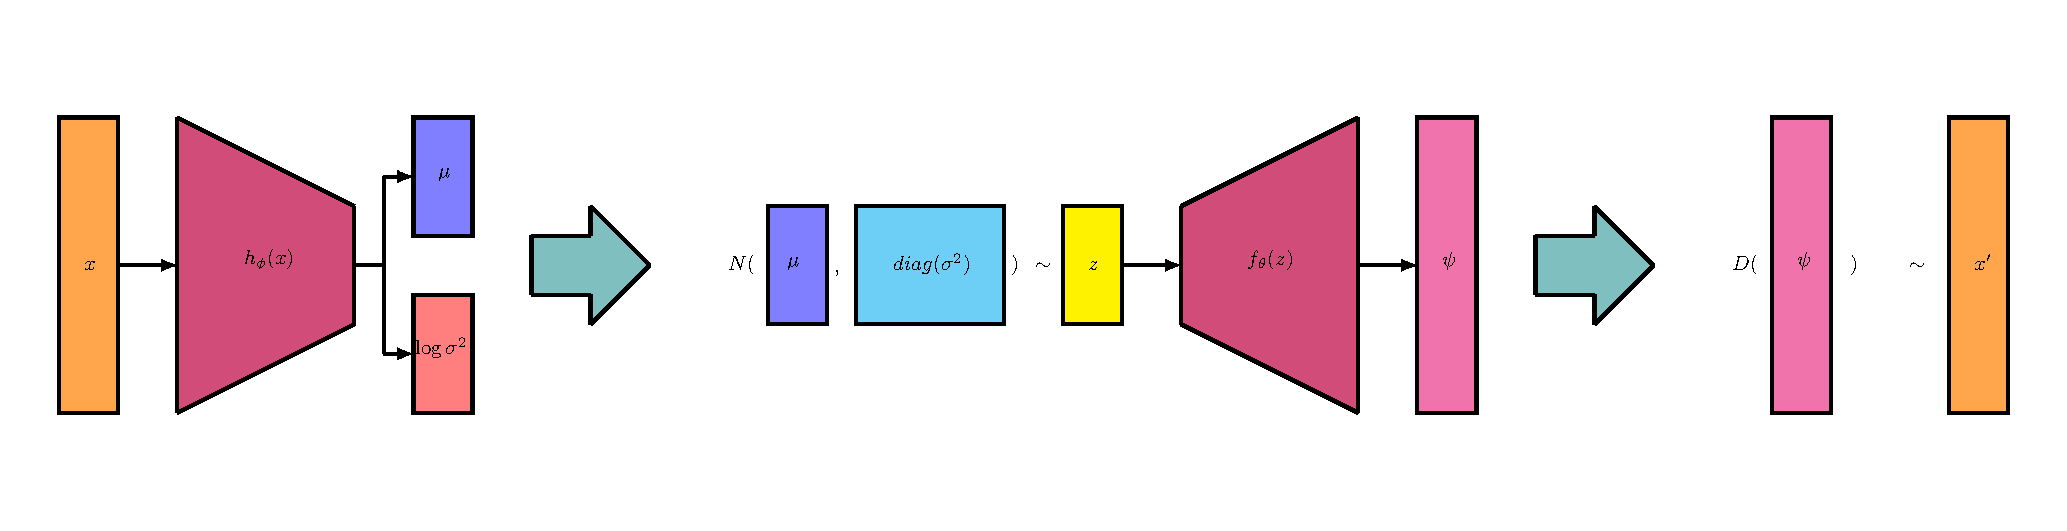
\includegraphics[width=\textwidth]{TIKZ_TEX_FILE/PDFS/high_vae.pdf}
    \caption{High-level block diagram of a Variational Autoencoder.}
    \label{fig:vae_block_diagram}
\end{figure}

\subsubsection{Decoder and Reconstruction}
The decoder reconstructs the original data \( x \) by mapping the latent variable \( z \) back to the input space. It achieves this by modeling a conditional probability distribution:
\[
p_\theta(x|z)
\]
where \( \theta \) represents the decoder's parameters. \\

The reconstructed output is trained to closely match the input, ensuring the latent representation captures essential features of the data. Reconstruction quality is measured using reconstruction loss, discussed later in Section.

\paragraph{Output:} The output layer generates data with the same dimensions as the input, completing the generative cycle of the VAE.

\begin{figure}[H]
    \centering
    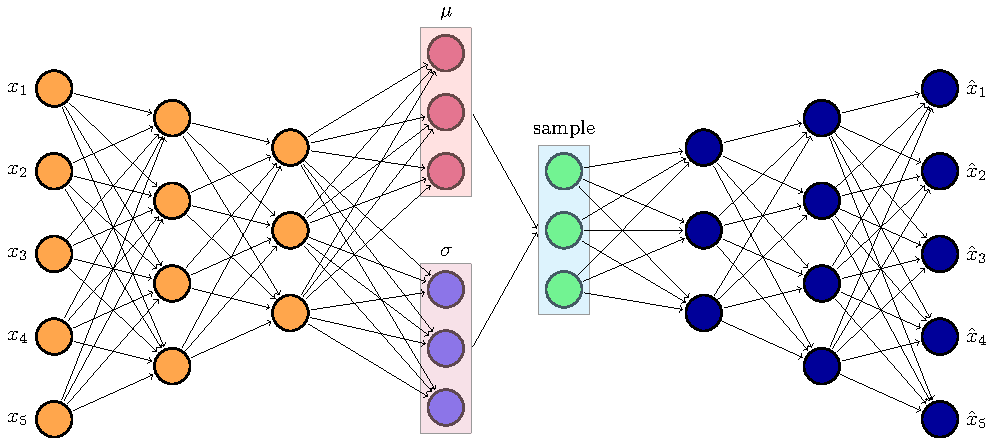
\includegraphics[width=\textwidth]{TIKZ_TEX_FILE/PDFS/vae_nn.pdf}
    \caption{Neural network representation of a Variational Autoencoder.}
    \label{fig:vae_nn_diagram}
\end{figure}


\section{Key Techniques in Variational Autoencoders}
\subsection{Reconstruction Loss}

Reconstruction loss plays a vital role in Variational Autoencoders (VAEs), ensuring that the decoder accurately reconstructs the input data from the latent variable. This section outlines the key components of reconstruction loss.

\subsubsection{Definition}

Reconstruction loss quantifies the discrepancy between the original input, $\mathbf{x}$, and its reconstructed counterpart, $\hat{\mathbf{x}}$, generated by the decoder. It is commonly expressed as:
\[
\mathcal{L}_{\text{recon}} = \mathbb{E}_{\mathbf{x} \sim p_{\text{data}}(\mathbf{x})} \left[ -\log p_{\theta}(\mathbf{x}|\mathbf{z}) \right],
\]
where $\mathbf{z} \sim q_{\phi}(\mathbf{z}|\mathbf{x})$ represents the latent variable sampled from the learned posterior.

\subsubsection{Loss Function Types}

The choice of the reconstruction loss function depends on the type of data:
\begin{itemize}
    \item \textbf{Cross-Entropy Loss}: Suitable for binary or categorical data.
    \item \textbf{Mean Squared Error (MSE)}: Appropriate for continuous data.
\end{itemize}

\subsubsection{Optimization Objective}

The goal of minimizing reconstruction loss is to optimize the decoder parameters $p_{\theta}(\mathbf{x}|\mathbf{z})$, enabling accurate recovery of input data. This is achieved through gradient descent, which adjusts both the encoder $q_{\phi}(\mathbf{z}|\mathbf{x})$ and decoder $p_{\theta}(\mathbf{x}|\mathbf{z})$ networks.

\subsubsection{Limitations}

While reconstruction loss ensures accurate reconstruction, it does not enforce structure on the latent space $\mathbf{z}$. This limitation necessitates the introduction of a regularization term, such as Kullback-Leibler divergence, to shape the latent space for generative purposes.



\subsection{KL Divergence as a Regularization Term}

\subsubsection{Need for Regularization in VAEs}
Discuss the limitations of relying solely on reconstruction loss for variational inference, emphasizing its failure to enforce structure in the latent space. Introduce the concept of continuity and completeness as desired properties of the latent space.

\subsubsection{Mathematical Definition of KL Divergence}
Present the mathematical expression for KL divergence:
\begin{equation}
    \mathcal{D}_{\text{KL}}(q_{\phi}(z|x) \,||\, p(z)) = \mathbb{E}_{q_{\phi}(z|x)} \left[ \log \frac{q_{\phi}(z|x)}{p(z)} \right]
\end{equation}
Define \( q_{\phi}(z|x) \) as the approximate posterior and \( p(z) \) as the prior distribution. Explain the intuition behind KL divergence as a measure of dissimilarity between these distributions.

\subsubsection{Role of KL Divergence in Latent Space Regularization}
Discuss how KL divergence addresses the two key properties of latent space:
\begin{itemize}
    \item \textbf{Continuity:} Ensures that latent space exhibits smooth transitions, meaning nearby points correspond to similar reconstructions.
    \item \textbf{Completeness:} Encourages the latent space to represent the full distribution, allowing for meaningful reconstructions even from unseen points.
\end{itemize}

\begin{figure}[h]
    \centering
    \includegraphics[width=\linewidth]{img/variational-autoencoder-distribution.png}
    \caption{Examples of how reconstruction loss and KL divergence affect the modeling of latent space for handwritten digits of 0-9 from the MNIST dataset.}
    \label{fig:enter-label}
\end{figure}


\subsection{Evidence Lower Bound (ELBO) and Its Derivation}

One obstacle to using KL divergence for variational inference is that the denominator of the posterior distribution $p(\mathbf{z}|\mathbf{x})$ is intractable. Variational Autoencoders (VAEs) address this challenge by approximating the minimization of KL divergence through the maximization of the Evidence Lower Bound (ELBO).

\subsubsection{Intuition of the ELBO}
In statistical terminology:
\begin{itemize}
    \item The \textbf{evidence} refers to $p(\mathbf{x})$, the marginal likelihood of the observed data $\mathbf{x}$.
    \item The \textbf{lower bound} refers to a worst-case estimate of the log-likelihood of the data.
\end{itemize}
Since directly computing the log-likelihood $\log p(\mathbf{x})$ is infeasible, the ELBO provides a tractable lower bound that can be optimized. \\ 

Maximizing the ELBO serves two purposes:
\begin{enumerate}
    \item It \textbf{maximizes the likelihood} of reconstructing the input data given the latent variables.
    \item It \textbf{minimizes the KL divergence} between the approximate posterior $q(\mathbf{z}|\mathbf{x})$ and the prior $p(\mathbf{z})$, ensuring smooth and structured latent space representations.
\end{enumerate}

\subsubsection{ELBO Derivation}
The starting point is the marginal log-likelihood $\log p(\mathbf{x})$. We derive the ELBO as follows:

\begin{align*}
\log p(\mathbf{x}) 
&= \log \int p(\mathbf{x}, \mathbf{z}) \, d\mathbf{z} \\
&= \log \int p(\mathbf{x}, \mathbf{z}) \frac{q(\mathbf{z}|\mathbf{x})}{q(\mathbf{z}|\mathbf{x})} \, d\mathbf{z} \quad \text{(introducing $q(\mathbf{z}|\mathbf{x})$)} \\
&\geq \mathbb{E}_{q(\mathbf{z}|\mathbf{x})} \left[ \log \frac{p(\mathbf{x}, \mathbf{z})}{q(\mathbf{z}|\mathbf{x})} \right] \quad \text{(Jensen's inequality)} \\
&= \mathbb{E}_{q(\mathbf{z}|\mathbf{x})} \left[ \log \frac{p(\mathbf{x}|\mathbf{z}) p(\mathbf{z})}{q(\mathbf{z}|\mathbf{x})} \right] \quad \text{(joint distribution factorization)} \\
&= \mathbb{E}_{q(\mathbf{z}|\mathbf{x})} \left[ \log p(\mathbf{x}|\mathbf{z}) \right] 
+ \mathbb{E}_{q(\mathbf{z}|\mathbf{x})} \left[ \log \frac{p(\mathbf{z})}{q(\mathbf{z}|\mathbf{x})} \right] \\
&= \mathbb{E}_{q(\mathbf{z}|\mathbf{x})} \left[ \log p(\mathbf{x}|\mathbf{z}) \right] 
- D_{\text{KL}} \left( q(\mathbf{z}|\mathbf{x}) \| p(\mathbf{z}) \right).
\end{align*}

Here:
\begin{itemize}
    \item $q(\mathbf{z}|\mathbf{x})$ is the approximate posterior, modeled by the encoder network.
    \item $p(\mathbf{x}|\mathbf{z})$ is the likelihood of reconstructing the data $\mathbf{x}$ from the latent variable $\mathbf{z}$, modeled by the decoder network.
    \item $p(\mathbf{z})$ is the prior distribution, typically assumed to be a standard multivariate Gaussian $\mathcal{N}(\mathbf{0}, \mathbf{I})$.
    \item $D_{\text{KL}}$ is the Kullback-Leibler divergence, which measures the discrepancy between the posterior and prior distributions.
\end{itemize}

Thus, the ELBO can be expressed as:
\[
\mathcal{L}(\theta, \phi) = \mathbb{E}_{q(\mathbf{z}|\mathbf{x})} \left[ \log p(\mathbf{x}|\mathbf{z}) \right] - D_{\text{KL}} \left( q(\mathbf{z}|\mathbf{x}) \| p(\mathbf{z}) \right),
\]
where:
\begin{itemize}
    \item The first term $\mathbb{E}_{q(\mathbf{z}|\mathbf{x})} \left[ \log p(\mathbf{x}|\mathbf{z}) \right]$ represents the reconstruction likelihood and encourages the VAE to reconstruct the input data accurately.
    \item The second term $D_{\text{KL}} \left( q(\mathbf{z}|\mathbf{x}) \| p(\mathbf{z}) \right)$ regularizes the latent space, ensuring that the approximate posterior $q(\mathbf{z}|\mathbf{x})$ remains close to the prior $p(\mathbf{z})$.
\end{itemize}

% \subsubsection{ELBO Components in Detail}
% \begin{itemize}
%     \item \textbf{Likelihood Term}: The term $\log p(\mathbf{x}|\mathbf{z})$ measures how well the latent variable $\mathbf{z}$ reconstructs the input $\mathbf{x}$. For binary input data, this likelihood is typically modeled as a Bernoulli distribution, leading to a cross-entropy loss:
%     \[
%     \log p(\mathbf{x}|\mathbf{z}) = \sum_{i=1}^n \left[ x_i \log \hat{x}_i + (1 - x_i) \log (1 - \hat{x}_i) \right],
%     \]
%     where $\hat{x}_i$ is the reconstructed pixel value.

%     \item \textbf{KL Divergence Term}: The KL divergence term $D_{\text{KL}} \left( q(\mathbf{z}|\mathbf{x}) \| p(\mathbf{z}) \right)$ ensures that the posterior $q(\mathbf{z}|\mathbf{x})$ remains close to the prior $p(\mathbf{z})$. For two Gaussian distributions, the KL divergence has a closed-form solution:
%     \[
%     D_{\text{KL}} \left( \mathcal{N}(\mu, \sigma^2) \| \mathcal{N}(0, 1) \right) = -\frac{1}{2} \sum_{j=1}^d \left( 1 + \log \sigma_j^2 - \mu_j^2 - \sigma_j^2 \right).
%     \]
% \end{itemize}

\subsection{Reparameterization Trick}

The goal of variational inference is to output new data as random variations of the training data $\mathbf{x}$. At first glance, this might seem straightforward: we could use a function $f$ to select a random value for the latent variable $\mathbf{z}$, which the decoder would then use to reconstruct $\mathbf{x}$. However, a fundamental problem arises: \textbf{randomness cannot be directly optimized}. \\

By definition, a vector of random values has no derivative—no gradient that expresses patterns in the resultant outputs—so it cannot be optimized using backpropagation. Without gradients, the neural network cannot learn the optimal parameters required to achieve its task. \\

To circumvent this issue, VAEs use the \textbf{reparameterization trick}. Instead of directly sampling $\mathbf{z}$ from the posterior $q(\mathbf{z}|\mathbf{x})$, we introduce an auxiliary random variable $\epsilon$, which is sampled from a standard normal distribution $\mathcal{N}(\mathbf{0}, \mathbf{I})$. The latent variable $\mathbf{z}$ is then reparameterized as:
\[
\mathbf{z} = \mu(\mathbf{x}) + \sigma(\mathbf{x}) \odot \epsilon, \quad \epsilon \sim \mathcal{N}(\mathbf{0}, \mathbf{I}),
\]
where:
\begin{itemize}
    \item $\mu(\mathbf{x})$ represents the mean of the approximate posterior, and  
    \item $\sigma(\mathbf{x})$ represents the standard deviation (or scale).  
\end{itemize} 

Here, $\epsilon$ introduces the stochasticity required for sampling, while $\mu$ and $\sigma$ are outputs of the encoder network. \\

In simpler terms, $\mathbf{z}$ starts at its mean $\mu(\mathbf{x})$ and is shifted by a random multiple of its standard deviation $\sigma(\mathbf{x})$. This reparameterization allows the random noise $\epsilon$ to remain independent of the model’s parameters, enabling gradients to propagate through $\mu$ and $\sigma$ during backpropagation. The model can then be optimized using standard gradient descent algorithms—most commonly Adam.

\subsection{Summary of the VAE Training Objective}

The training objective for VAEs is to maximize the Evidence Lower Bound (ELBO):
\[
\mathcal{L}(\theta, \phi) = \mathbb{E}_{q(\mathbf{z}|\mathbf{x})} \left[ \log p(\mathbf{x}|\mathbf{z}) \right] - D_{\text{KL}} \left( q(\mathbf{z}|\mathbf{x}) \| p(\mathbf{z}) \right),
\]
where:
\begin{itemize}
    \item The first term ensures accurate reconstruction of the input data $\mathbf{x}$.
    \item The second term regularizes $q(\mathbf{z}|\mathbf{x})$ to stay close to the prior $p(\mathbf{z})$.
\end{itemize}

The reparameterization trick enables backpropagation through the sampling process, making the ELBO optimizable via gradient descent.


\section{Comparison Between Autoencoders and Variational Autoencoders}

The key differences between standard Autoencoders (AEs) and Variational Autoencoders (VAEs) are summarized in the following Table

\begin{table}[H]
\centering
\small
\renewcommand{\arraystretch}{1.6} % Increases row spacing
\setlength{\tabcolsep}{12pt} % Adjusts column spacing
\label{tab:ae_vs_vae}
\begin{tabular}{|p{0.2\textwidth}||p{0.35\textwidth}|p{0.35\textwidth}|}
\hline
 \textbf{Aspect} & \textbf{Standard Autoencoder} & \textbf{Variational Autoencoder} \\ \hline

\textbf{Latent Space} & Deterministic: Each input maps to a fixed latent vector. & Probabilistic: Each input maps to a distribution characterized by a mean \( \mu \) and variance \( \sigma^2 \). \\ \hline

 \textbf{Loss Function} & Minimizes reconstruction error, such as Mean Squared Error (MSE) or cross-entropy. & Minimizes the Evidence Lower Bound (ELBO) \\ \hline

\textbf{Regularization} & No explicit regularization of the latent space. & Regularizes the latent space to follow a prior distribution, typically \( \mathcal{N}(0, 1) \). \\ \hline

 \textbf{Generative Nature} & Non-generative: Cannot sample new data. & Generative: Capable of sampling new data points by sampling latent vectors \( \mathbf{z} \sim \mathcal{N}(\mu, \sigma^2) \). \\ \hline

\textbf{Philosophy} & Encodes and decodes inputs deterministically for compression or reconstruction. & Bayesian approach: Learns a probabilistic model of the data distribution \( p(\mathbf{x}, \mathbf{z}) \). \\ \hline

 \textbf{Applications} & Compression, denoising, and feature extraction. & Generative modeling, anomaly detection, and smooth latent space interpolation. \\ \hline
\end{tabular}
\caption{Key Differences Between Autoencoders and Variational Autoencoders}
\end{table}

In summary, while standard autoencoders are well-suited for tasks like compression and feature extraction, VAEs introduce a probabilistic framework that enables generative capabilities.

\section{Conditional Variational Autoencoders (CVAE)}

\subsection{Limitations of Vanilla VAE}
One significant shortcoming of conventional \textbf{vanilla VAEs} is that they offer \textbf{no control} over the specific outputs generated. For instance:  
\begin{itemize}
    \item A vanilla VAE trained on the \textbf{MNIST dataset} will generate random handwritten digits ranging from 0 to 9.
    \item However, it cannot be constrained to generate digits \textbf{only 4s or 7s}.
\end{itemize}
This lack of control limits their applicability in tasks where specific outputs based on certain conditions are desired.

\subsection{Advantages of Conditional VAE (CVAE)}
Conditional Variational Autoencoders (CVAEs) address the limitations of vanilla VAEs by enabling \textbf{controlled outputs} conditioned on specific inputs. This is achieved by incorporating elements of supervised learning alongside the unsupervised objectives of standard autoencoders.

\begin{itemize}
    \item Instead of generating purely random variations, CVAEs condition the generation process on \textbf{labels or attributes}.
    \item For example, when trained on the MNIST dataset, a CVAE can generate specific digits, such as \textbf{4s or 7s}, by conditioning on the desired class label.
\end{itemize}

\subsection{Comparison Between Vanilla VAE and CVAE}
\begin{table}[H]
    \centering
    \renewcommand{\arraystretch}{1.6} % Increases row spacing
    \label{tab:vae_cvae_comparison}
    \begin{tabular}{|p{8cm}|p{8cm}|}
        \hline
        \textbf{\hspace{5em} Vanilla VAE} & \textbf{\hspace{5em} Conditional VAE} \\ \hline
        Generates random outputs with no control. & Generates outputs conditioned on specific inputs (e.g., labels). \\ \hline
        Purely unsupervised learning. & Incorporates elements of supervised learning alongside unsupervised learning. \\ \hline
        Cannot generate targeted outputs (e.g., only digits 4 or 7 in MNIST). & Enables controlled generation of specific outputs (e.g., only digits 4 or 7). \\ \hline
        Limited applicability in tasks requiring precise control. & Useful in class-conditional or attribute-specific generation tasks. \\ \hline
    \end{tabular}
    \caption{Comparison of Vanilla VAE and CVAE}
\end{table}

\subsection{Comparison Block Diagram}
\begin{figure}[H]
    \centering
    % Placeholder for your diagram
    \includegraphics[width=0.8\linewidth]{img/cvae.png}
    \caption{Comparison of Vanilla VAE and Conditional VAE}
    \label{fig:vae_cvae_diagram}
\end{figure}

\section{More Generative Models}

Generative models are designed to learn the underlying distribution of data and generate new data points that resemble the original dataset. Autoencoders, a class of neural networks, serve as the foundational architecture for several advanced generative models. Below, we highlight some key generative models based on autoencoders.

\subsection{Notable Generative Models Using Autoencoders}

Several generative models leverage the autoencoder architecture to model data distributions. Some of the prominent models include:

\begin{itemize}
    \item \textbf{Variational Autoencoders (VAEs):} VAEs extend traditional autoencoders by incorporating probabilistic components, allowing them to model complex distributions and generate new data points.
    \item \textbf{Conditional Variational Autoencoders (CVAEs):} Building upon VAEs, CVAEs condition the generation process on additional information, enabling more controlled generation.
    \item \textbf{Masked Autoencoders for Distribution Estimation (MADE):} MADE utilizes a masking mechanism to model the distribution of data in an autoregressive manner, making it efficient for high-dimensional data.
    \item \textbf{Adversarial Autoencoders (AAEs):} AAEs combine autoencoders with generative adversarial networks (GANs), introducing adversarial training to improve the quality of generated samples.
\end{itemize}

\subsection{MADE (Masked Autoencoder for Distribution Estimation)}

Among the models mentioned, MADE is particularly noteworthy due to its innovative use of a \textbf{masking mechanism} for efficient distribution estimation. By leveraging the autoregressive nature of data, MADE learns complex dependencies between variables in a data set and is capable of generating new samples from the learned distribution.

\subsection{Key Aspects of MADE}

\begin{itemize}
    \item \textbf{Masking Mechanism:} The model uses a masking strategy that enables it to learn distributions effectively, particularly when dealing with high-dimensional data.
    \item \textbf{Generative Model:} Once trained, MADE can generate new samples by drawing from the distribution it has learned.
    \item \textbf{Autoregressive Nature:} MADE models dependencies in a sequential, autoregressive manner, allowing it to capture the relationships between different variables.
\end{itemize}

% Insert TikZ diagram of MADE here
\begin{figure}[H]
    \centering
    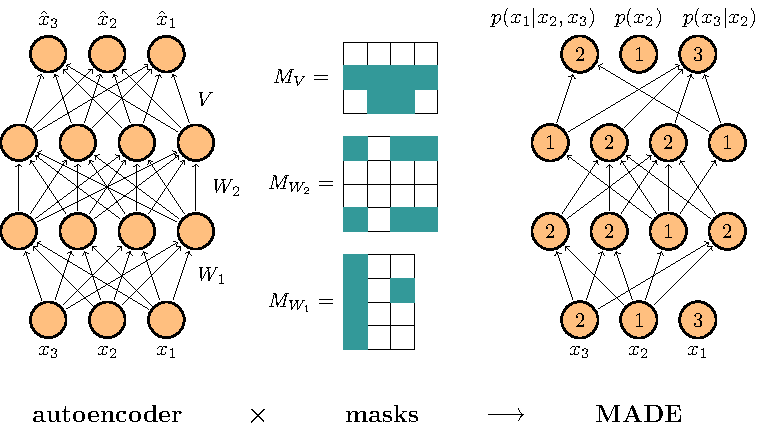
\includegraphics[width=0.8\textwidth]{TIKZ_TEX_FILE/PDFS/made_pdf.pdf} % Replace with your actual diagram
    \caption{MADE (Masked Autoencoder for Distribution Estimation) Diagram.}
\end{figure}

\section{Limitations and Future Prospects}

\subsection{Challenges in Generative Autoencoders}
Generative autoencoders, while powerful, face several limitations that impact their performance and scalability. Some of the primary challenges include:
\begin{itemize}
    \item \textbf{Scalability:} As data dimensions grow, training generative autoencoders becomes increasingly difficult, requiring vast computational resources.
    \item \textbf{Training Instability:} Autoencoders, particularly in complex models like VAEs or GAN-based architectures, often suffer from issues such as non-convergence or poor-quality samples.
    \item \textbf{Mode Collapse:} This issue is common in generative models, where the model fails to capture the full diversity of the data distribution, generating only a limited set of samples.
    \item \textbf{Lack of Interpretability:} Despite being effective in generating data, the models are often considered "black boxes," making it hard to understand the reasons behind their decisions or generated outputs.
\end{itemize}

\subsection{Role of Conditional and Masked Models}
Conditional and masked models, such as Conditional Variational Autoencoders (CVAEs) and Masked Autoencoders for Distribution Estimation (MADE), offer solutions to some of the challenges faced by traditional generative autoencoders:
\begin{itemize}
    \item \textbf{Enhanced Flexibility:} Conditional models allow the generation of data conditioned on certain inputs, improving control over the generated outcomes.
    \item \textbf{Masking for Efficiency:} Masked autoencoders like MADE improve learning efficiency by introducing a masked structure that helps capture dependencies in high-dimensional data more effectively.
    \item \textbf{Better Data Utilization:} These models ensure that every piece of input data is efficiently utilized, addressing scalability issues by focusing on more relevant features.
\end{itemize}

\subsection{Future Directions in Generative Modeling}
The future of generative autoencoders is promising, with numerous areas for improvement and exploration:
\begin{itemize}
    \item \textbf{Increased Scalability:} With advancements in hardware and optimization techniques, generative models will be better equipped to handle large-scale datasets and complex problems.
    \item \textbf{Improved Training Stability:} New algorithms and methods to stabilize the training of generative models, including regularization techniques and better loss functions, will likely emerge, addressing common issues like mode collapse and non-convergence.
    \item \textbf{Interpretable Models:} There is a growing demand for more interpretable generative models, where the reasoning behind generated outputs can be understood, leading to broader adoption in sensitive applications.
    \item \textbf{Multi-modal Generation:} The integration of different types of data, such as text, image, and audio, will be an area of intense research, enabling generative models to handle complex multi-modal tasks.
\end{itemize}


%%%%%%%%%%%%%%%%%%%%%%%%%%%%%%%%%%%%%%%%%%%%%%%%%%%%%%%%%%%%%%%%%%%%%%%%%%%%%%%%%%%%%%%%%%%%%%%
                                    % FARIHA IFRAT %
%%%%%%%%%%%%%%%%%%%%%%%%%%%%%%%%%%%%%%%%%%%%%%%%%%%%%%%%%%%%%%%%%%%%%%%%%%%%%%%%%%%%%%%%%%%%%%%

\section{Overview of Denoising Autoencoders}

Denoising autoencoders (DAEs) are a class of neural networks designed to learn robust representations of data by reconstructing clean data from noisy or corrupted inputs. These models are particularly effective at denoising data and have shown their value in various fields. Below are some key aspects of denoising autoencoders:

\begin{itemize}
    \item Denoising autoencoders aim to remove noise from corrupted data and reconstruct the original, clean data.
    \item These models are widely used in fields such as image denoising, speech enhancement, and data recovery, where data is often noisy or incomplete.
\end{itemize}

\section{Mechanism and Functionality}

The core functionality of denoising autoencoders involves training the model to denoise and reconstruct data through a process of corruption and learning. The mechanism behind their success is outlined as follows:

\begin{itemize}
    \item Noisy data is created by adding artificial noise to the input, simulating the process of data corruption in real-world applications.
    \item The autoencoder is trained to learn how to reconstruct the original, clean version of the input data, using the noisy version as the input.
    \item The network learns to capture a compressed, noise-invariant representation in the bottleneck layer, which can be used to recover the original data.
\end{itemize}



\section{Architecture of a Denoising Autoencoder}
   \begin{center}

   \begin{tikzpicture}[
    font=\sffamily,
    encoder/.style={trapezium, draw=blue!70, fill=blue!20, thick, minimum width=2cm, minimum height=1.2cm, rotate=270},
    decoder/.style={trapezium, draw=orange!70, fill=orange!20, thick, minimum width=2cm, minimum height=1.2cm, rotate=90},
    bottleneck/.style={rectangle, draw=purple!70, fill=purple!20, thick, minimum width=1.2cm, minimum height=1.2cm},
    arrow/.style={thick,->},
    image/.style={inner sep=0pt, anchor=center}
]


% Input Image
\node[image] (x) {\includegraphics[width=1.5cm]{Encoder/NoisyPic.png}};
\node[above=0.4cm of x, font=\small, align=center, text=blue!100] {\textbf{Input}};
\node[below=0.5cm of x, font=\small, text=blue!100] {$\mathbf{x}$};

% Encoder
\node[encoder, right=1.8cm of x] (encoder) {};
\node[above=0.4cm of encoder, font=\small, align=center, text=blue!100] {\textbf{Encoder }\\ $\mathbf{g_\phi}$};
\draw[arrow] (x) -- (encoder);

% Bottleneck
\node[bottleneck, right=1.8cm of encoder] (z) {$\mathbf{z}$};
\node[above=0.4cm of z, font=\small, align=center, text=purple!100] {\textbf{Bottleneck}};
\node[below=0.6cm of z, text width=3cm, align=center, font=\small, text=purple!70]{A compressed low \\ dimensional representation \\ of the input.};
\draw[arrow] (encoder) -- (z);

% Decoder
\node[decoder, right=1.8cm of z] (decoder) {};
\node[above=0.4cm of decoder, font=\small, align=center, text=orange!100] {\textbf{Decoder }\\ $\mathbf{f_\theta}$};
\draw[arrow] (z) -- (decoder);

% Reconstructed Image
\node[image, right=1.8cm of decoder] (x_prime) {\includegraphics[width=1.5cm]{Encoder/denoisedPic.png}};
\node[above=0.4cm of x_prime, font=\small, align=center, text=orange!70] {\textbf{Output}};
\node[below=0.5cm of x_prime, font=\small, text=orange!100] {$\mathbf{x'}$};
\draw[arrow] (decoder) -- (x_prime);

% Dashed line (ideally identical)
\node[above=0.3cm of x.east, xshift=4.5cm, font=\small, align=center, text=gray!70] {Ideally, they are identical: \\ $\mathbf{x} \approx \mathbf{x'}$};

\end{tikzpicture}
\end{center}
\raggedright
\subsection{Encoder ($g_\phi$)}
The encoder is the first stage of the denoising autoencoder. Its primary responsibility is to transform the noisy input data ${x}$ into a latent representation $z$, which is both compact and robust to noise. This transformation involves multiple learnable layers, such as fully connected layers or convolutional layers, depending on the data type. The parameters of the encoder, $\phi$, are optimized during training to ensure meaningful feature extraction.

\begin{itemize}
    \item \textbf{Input:} Noisy data $\tilde{x}$, which contains artificially introduced corruption (e.g., Gaussian noise).
    \item \textbf{Transformation:} The encoder applies nonlinear transformations using activation functions (e.g., ReLU or sigmoid) to extract hierarchical features.
    \item \textbf{Output:} A latent vector $z$, representing noise-invariant, compressed features crucial for data reconstruction.
    \item \textbf{Role in Denoising:} By extracting the essential characteristics of the data, the encoder effectively separates the signal from the noise.
\end{itemize}
\subsection{Bottleneck ($z$)}
The bottleneck is a critical component of the autoencoder architecture. It serves as the intermediate layer where the data is represented in a compressed form. This compressed representation enables the autoencoder to focus on the most relevant features while ignoring noise and redundancy.

\begin{itemize}
    \item \textbf{Dimensionality Reduction:} The bottleneck layer has a significantly smaller dimensionality compared to the input data. This forces the model to encode only the most salient features.
    \item \textbf{Noise Robustness:} The compression inherently filters out noise, as irrelevant details are not preserved in the reduced representation.
    \item \textbf{Key Functionality:} The bottleneck enables generalization and ensures the decoder can reconstruct the clean data without retaining the noise.
\end{itemize}

\subsection{Decoder ($f_\theta$)}
The decoder reverses the operations of the encoder. Its task is to reconstruct the clean data $x$ from the compressed latent representation $z$. The decoder learns a mapping from the latent space back to the original data space, ensuring that the output $\hat{x}$ closely resembles the original input $x$.

\begin{itemize}
    \item \textbf{Input:} Latent representation $z$, which contains the core features of the data.
    \item \textbf{Transformation:} The decoder applies a series of operations (e.g., upsampling, deconvolutions, or fully connected layers) to map $z$ back to the data space.
    \item \textbf{Output:} The reconstructed data $\hat{x}$, which approximates the clean version of the input data.
    \item \textbf{Role in Denoising:} By learning to reconstruct only the original clean signal, the decoder ensures the elimination of noise introduced in the input.
\end{itemize}

\subsection{Overall Workflow}
The overall workflow involves the \textbf{encoder} compressing noisy input into a latent representation, the \textbf{bottleneck layer} focusing on core features, and the \textbf{decoder} reconstructing the clean data. This process minimizes the reconstruction error and ensures that the model effectively removes noise while preserving the original data structure.

\section{Mathematical Foundation}

Denoising autoencoders rely on a well-defined mathematical framework to achieve effective noise removal while retaining the essential characteristics of the input data. The key components of this foundation are outlined below:
\subsection{Encoding and Decoding Process}
The mathematical operations of the encoder and decoder can be described as follows:

\begin{itemize}
    \item \textbf{Encoding:} The encoder applies a nonlinear transformation to map the noisy input $\tilde{x}$ to a latent representation $z$:
    \begin{equation}
        z = g_\phi(\tilde{x}),
    \end{equation}
    where $g_\phi$ is the encoding function parameterized by $\phi$.
    
    \item \textbf{Decoding:} The decoder reconstructs the clean data $\hat{x}$ from the latent representation $z$:
    \begin{equation}
        \hat{x} = f_\theta(z),
    \end{equation}
    where $f_\theta$ is the decoding function parameterized by $\theta$.
\end{itemize}

\subsection{Regularization and Noise Modeling}
Adding noise to the input data $\tilde{x}$ plays a critical role in the denoising process. Noise is modeled as a random perturbation $\eta$ added to the clean input:
\begin{equation}
    \tilde{x} = x + \eta,
\end{equation}
where $\eta$ is sampled from a noise distribution (e.g., Gaussian noise or salt-and-pepper noise).

This regularization forces the autoencoder to focus on extracting meaningful features from the data, rather than memorizing noise patterns.

\subsection{Optimization}
Training the autoencoder involves optimizing the parameters $\phi$ (encoder) and $\theta$ (decoder) to minimize the reconstruction loss. Gradient-based optimization methods, such as Stochastic Gradient Descent (SGD) or Adam, are typically employed. The parameter update rule is given by:

\begin{equation}
    \phi, \theta \leftarrow \phi, \theta - \eta \cdot \nabla_{\phi, \theta} \mathcal{L}(x, \hat{x}),
\end{equation}

where $\eta$ is the learning rate and $\nabla_{\phi, \theta} \mathcal{L}$ is the gradient of the loss function with respect to the model parameters.
\subsection{Loss Function}
The reconstruction error is quantified using a loss function, which measures the discrepancy between the clean input and the reconstructed output. Typically, the Mean Squared Error (MSE) is used:

\begin{equation}
    \mathcal{L}(x, \hat{x}) = \frac{1}{N} \sum_{i=1}^N \|x_i - \hat{x}_i\|^2,
\end{equation}

where:
\begin{itemize}
    \item $x_i$: The $i$-th sample of the clean input data.
    \item $\hat{x}_i$: The $i$-th sample of the reconstructed data.
    \item $N$: The total number of samples.
\end{itemize}

The loss function encourages the model to minimize the reconstruction error, effectively removing the added noise while preserving the data's original features.

\subsection{Reconstruction Accuracy Metrics}
To evaluate the performance of the autoencoder, the following metrics are commonly used:
\begin{itemize}
    \item \textbf{Peak Signal-to-Noise Ratio (PSNR):} Measures the quality of reconstruction relative to the noise level.
    \item \textbf{Structural Similarity Index Measure (SSIM):} Assesses the perceptual similarity between the original and reconstructed data.
\end{itemize}
These metrics help quantify the effectiveness of the model in removing noise while preserving the original data's integrity.

\section{Training Process}

The training process of a denoising autoencoder involves encoding corrupted inputs to a latent representation and then reconstructing the original input as accurately as possible. This process aims to minimize the reconstruction error by iteratively adjusting the weights and biases of the network. The flowchart below illustrates the step-by-step mechanism of the training pipeline, while the accompanying algorithm provides a detailed explanation of the procedure.\\

\tikzstyle{startstop} = [rectangle, rounded corners, minimum width=3cm, minimum height=1cm, text centered, draw=black, fill=red!30,drop shadow]
\tikzstyle{process} = [rectangle, minimum width=3cm, minimum height=1cm, text centered, draw=black, fill=blue!30,drop shadow]
\tikzstyle{decision} = [diamond, minimum width=1.5cm, minimum height=0.5cm, text centered, draw=black, fill=green!30,drop shadow]
\tikzstyle{data} = [trapezium, trapezium left angle=70, trapezium right angle=110, minimum width=3cm, minimum height=1cm, text centered, draw=black, fill=orange!30,drop shadow]
\tikzstyle{arrow} = [thick,->,>=stealth]
\tikzstyle{connect} = [draw, thick, color=black, opacity=0.5]
\tikzset{
    neuron/.style={circle, draw=black, thick, minimum size=0.7cm, text centered, text=white, font=\small, fill=blue!70},
    encoder/.style={rectangle, draw=orange!60, thick, fill=orange!30, rounded corners, minimum width=2.5cm, text centered, font=\bfseries},
    decoder/.style={rectangle, draw=blue!60, thick, fill=blue!30, rounded corners, minimum width=2.5cm, text centered, font=\bfseries},
    noisy/.style={rectangle, draw=green!60, thick, fill=green!30, rounded corners, minimum width=2.5cm, text centered, font=\bfseries},
    output/.style={rectangle, draw=red!60, thick, fill=red!30, rounded corners, minimum width=2.5cm, text centered, font=\bfseries},
    arrow/.style={->, thick, >=stealth, draw=black!80},
    connect/.style={->, thick, draw=gray!80},
}


\centering
\vspace{0.5 cm }
\scalebox{.7}{
\begin{tikzpicture}[node distance=3cm and 3cm]
% Nodes
% Arrows
\node (samples) [data] {Training Samples};

\node (corrupted) [process, below of=samples] {Corrupted Input};
\draw [arrow] (samples) -- (corrupted);
\node (hidden) [process, below of=corrupted] {Hidden Layers (Feature Vector)};
\draw [arrow] (corrupted) -- (hidden);
\node (reconstruction) [data, below of=hidden] {Reconstruction Signals};
\draw [arrow] (hidden) -- (reconstruction);
\node (error) [decision, right of=corrupted, xshift=3cm, text width=2.5cm] {Minimizing Reconstruction Error};
\draw [arrow] (corrupted.east) -- ++(0.5,0) |- (error.west);
\node (fine) [startstop, below of=error] {Fine-tuning Weights};
\draw [arrow] (error) -- (fine);
\draw [arrow] (fine.west) -- ++(-0.5,0) |- (hidden.east);

\end{tikzpicture}
}
\vspace{1 cm}

\raggedright
The algorithm below outlines the detailed steps involved in training the denoising autoencoder, highlighting the iterative process of minimizing the reconstruction loss and updating the model parameters.

\begin{algorithm}
\caption{Training a Denoising Autoencoder}
\begin{algorithmic}[1]
\Require Dataset $\mathcal{D}$, learning rate $\eta$, number of epochs $E$.
\State Initialize parameters $\phi$, $\theta$.
\For{epoch $= 1, \dots, E$}
    \For{each mini-batch $\{x_1, \dots, x_m\} \subset \mathcal{D}$}
        \State Add noise: $\tilde{x}_i = x_i + \text{noise}$.
        \State Encode: $z_i = g_\phi(\tilde{x}_i)$.
        \State Decode: $\hat{x}_i = f_\theta(z_i)$.
        \State Compute loss: $\mathcal{L} = \frac{1}{m} \sum_{i=1}^m \|x_i - \hat{x}_i\|^2$.
        \State Update $\phi, \theta$ using gradient descent.
    \EndFor
\EndFor
\end{algorithmic}
\end{algorithm}
\raggedright
\section{Applications of Denoising Autoencoders}

Denoising autoencoders have widespread applications in various fields due to their ability to learn robust representations and remove noise from corrupted data. Some notable applications include:

\begin{itemize}
     \item \textbf{Pretraining for Neural Networks:} Using the learned features from denoising autoencoders as a starting point for training deeper neural networks, especially in cases with limited labeled data.
    
    \item \textbf{Image Denoising:} Removing noise from images to improve visual quality and restore clarity, especially in photography and medical imaging.
    \begin{figure}[H]
        \centering
        
\includegraphics[width=0.4\textwidth]{frames2/frame_2.png}
        
\includegraphics[width=0.4\textwidth]{frames2/frame_19.png}
        \caption{An example of image denoising using a denoising autoencoder. The noisy image is on the left, and the denoised image is on the right.}
        \label{fig:denoising}
    \end{figure}

    \item \textbf{Speech Enhancement:} Improving the quality of noisy audio signals, such as removing background noise from speech recordings.
    
    \item \textbf{Data Compression:} Learning compact and efficient representations of high-dimensional data, which can be used for storage and transmission.

    
     \item \textbf{Feature Extraction:} Extracting meaningful and noise-invariant features for downstream tasks like classification and clustering.

     
    \item \textbf{Anomaly Detection:} Identifying anomalies or outliers in datasets by measuring the reconstruction error, commonly used in fraud detection and network monitoring.
    \begin{figure}[H]
        \centering
        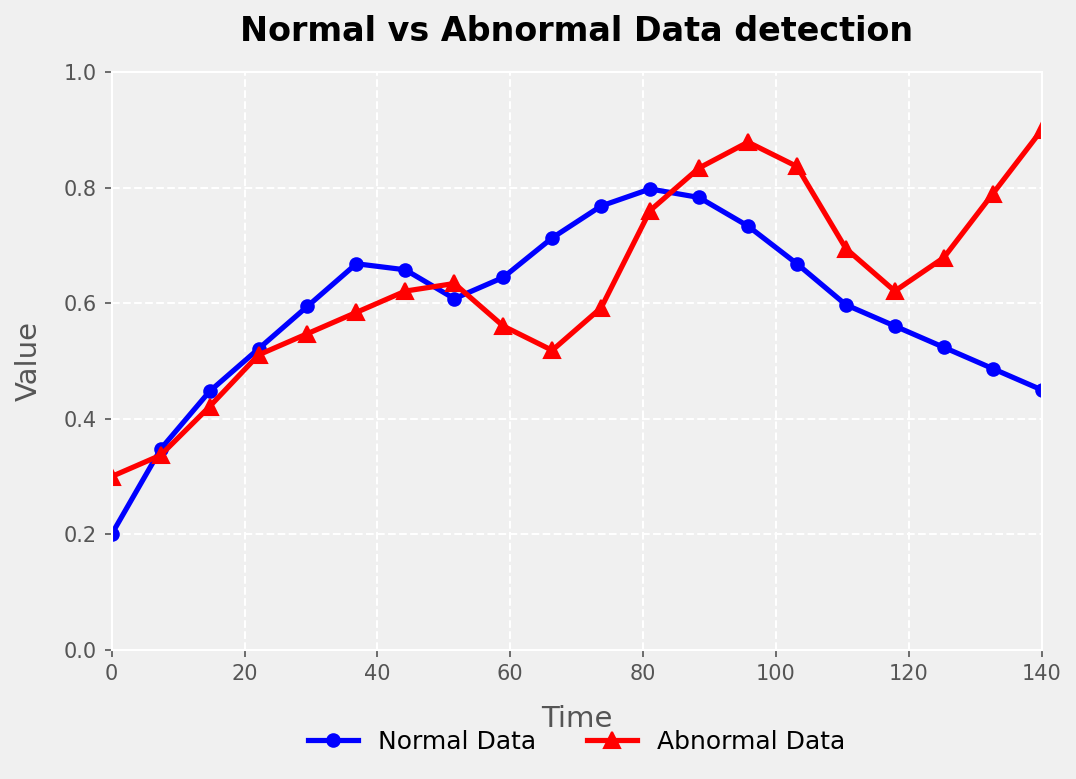
\includegraphics[width=0.6\textwidth]{frames/frame_19.png} % Replace with your image file
        \caption{Anomaly detection using a denoising autoencoder. The figure shows the reconstruction error, where anomalies can be identified by high reconstruction errors.}
        \label{fig:anomaly_detection}
    \end{figure}
   
\end{itemize}

Denoising autoencoders are pivotal in enhancing the quality and utility of data across diverse domains, serving as foundational components in modern machine learning pipelines.

\vspace{0.5 cm}
\section{Challenges and Advantages of Denoising Autoencoders}

Denoising autoencoders have proven useful in many applications, but there are both challenges and advantages to consider. The following table summarizes these points:
\vspace{0.3 cm}

\begin{table}[h!]
    \centering
    \renewcommand{\arraystretch}{1.6} % Increases row spacing
    \begin{tabular}{|p{6cm}|p{6cm}|}
    \hline
    \textbf{Challenges} & \textbf{Advantages} \\ \hline
    \textbf{High computational cost} & \textbf{Improved data quality} \\
    Training denoising autoencoders can be computationally expensive, especially for large datasets and deep models. & Denoising autoencoders can significantly improve data quality by removing noise from corrupted inputs. \\ \hline
    
    \textbf{Sensitive to noise levels} & \textbf{Versatility across domains} \\
    The performance of denoising autoencoders depends on the type and level of noise in the data. They may not perform well for extreme noise levels. & Denoising autoencoders are applicable to various domains like image processing, speech enhancement, and anomaly detection. \\ \hline
    \end{tabular}
    \label{tab:challenges_advantages_part1}
    \end{table}
    
    \newpage
    
    \begin{table}[h!]
    \centering
    \renewcommand{\arraystretch}{1.6} % Increases row spacing
    \begin{tabular}{|p{6cm}|p{6cm}|}
        \hline
        \textbf{Challenges} & \textbf{Advantages} \\ \hline
        \textbf{Risk of overfitting} & \textbf{Feature learning} \\
        Denoising autoencoders may overfit the training data, particularly with small datasets or excessive network complexity. & They are capable of learning robust features that generalize well to different tasks. \\ \hline
        
        \textbf{Requirement for large datasets} & \textbf{Pretraining for other models} \\
        Large labeled or unlabeled datasets are typically required for training effective denoising autoencoders. & Denoising autoencoders can be used for pretraining, providing useful feature representations for downstream tasks. \\ \hline
    \end{tabular}
    \caption{Challenges and Advantages of Denoising Autoencoders}
    \label{tab:challenges_advantages_part2}
    \end{table}
    

\section{Conclusion}

\justify 

Autoencoders have emerged as a cornerstone in the landscape of unsupervised machine learning, enabling significant advancements in data analysis, representation learning, and feature extraction. By compressing data into a lower-dimensional latent space and reconstructing it with minimal loss, they serve as powerful tools in various domains, including image and speech processing, anomaly detection, and data denoising. \\[1em]

One of the most impactful variations of autoencoders is the \textbf{Generative Autoencoder}, such as the \textbf{Variational Autoencoder (VAE)}, which goes beyond simple data reconstruction to generate entirely new data points from learned distributions. These models have become essential in areas like generative modeling, where they create realistic images, texts, and even audio, contributing to advancements in creative AI applications, data augmentation, and simulation-based tasks. The ability to generate new, plausible data has paved the way for their use in generative adversarial networks (GANs) and other creative endeavors, allowing for the synthesis of high-quality data in a way that mimics real-world distributions. \\[1em]

Another critical advancement is the \textbf{Denoising Autoencoder}, which focuses on reconstructing corrupted or noisy input data. By training on noisy datasets, denoising autoencoders learn to filter out noise and recover the underlying clean data. This capability has profound applications in fields such as image restoration, speech enhancement, and signal processing. In environments where data is often incomplete or distorted, denoising autoencoders offer solutions for improving data quality, leading to more robust machine learning models and better predictive accuracy. \\[1em]

Despite their successes, challenges remain. Issues like overfitting, the need for large amounts of labeled data, and computational resource demands still require attention. However, the continuous progress in regularization techniques, transfer learning, and more efficient training methodologies is making autoencoders more adaptable and scalable for real-world applications. \\[1em]

In conclusion, autoencoders are not merely a tool for dimensionality reduction; they represent a transformative class of models that are reshaping how we interact with data. With the rise of \textbf{Generative Autoencoders} and \textbf{Denoising Autoencoders}, these models are expanding their utility across diverse industries—from generating synthetic data for training purposes to improving the clarity of noisy inputs in critical systems. The future of autoencoders looks promising, with their capabilities continuing to evolve and drive innovation in fields ranging from healthcare diagnostics to autonomous systems and beyond. \\[1em]

\nocite{*}
\bibliography{ref.bib}

\end{document}
